
%\documentclass[10pt,letterpaper]{article}
%\usepackage{cogsci}

\documentclass[man,floatsintext]{apa6}

\usepackage[nodoi]{apacite}
\usepackage{graphicx, subcaption}
\usepackage{amsmath}
\usepackage[american]{babel}
\usepackage[section]{placeins}

\usepackage{soul} % for \hl
\usepackage{color}
%\renewcommand\bibliographytypesize{\footnotesize}
\usepackage{pslatex}
% \usepackage{multirow}

\title{Desirable difficulties in the development of active inquiry skills}
\shorttitle{Desirable difficulties in active inquiry}
\author{
 George Kachergis, Marjorie Rhodes, \& Todd Gureckis \\
  \{george.kachergis, marjorie.rhodes, todd.gureckis\}@nyu.edu \\
}
\affiliation{Department of Psychology \\
   New York University \\
  New York, NY
  }

\begin{document}

\maketitle

\begin{abstract}

This study explores developmental changes in the ability to ask 
informative questions, hypothesizing an intrinsic link between the ability to 
update beliefs in light of evidence and the ability to ask informative questions. 
Four- to ten-year-old children 
played an iPad game asking them to identify a hidden insect. Learners could either 
ask about individual insects, or make a series of feature queries (e.g., ``Does the 
hidden insect have antenna?'') that could more efficiently narrow the hypothesis 
space. Critically, the task display either helped children integrate evidence 
with the hypothesis space or required them to perform this operation themselves.  Although the results 
indicate that helping children update their beliefs improved some aspects of their active 
inquiry behavior, children required to update their own beliefs asked questions that 
were more context-sensitive and thus informative.  The results show how making a 
task more difficult may actually improve children's active inquiry skills, thus 
illustrating a type of desirable difficulty.

\textbf{Keywords:} 
question asking, information search, active inquiry, hypothesis testing, scientific 
reasoning
\end{abstract}


\section{Introduction} 

%Figuring out how to efficiently navigate a hypothesis space--
%from learning the diagnostic features to asking the appropriate questions to 
%appropriately updating the space in the face of new evidence--is an essential part of 
%science, and of life, in general. 
A central part of science--and life, in general--is figuring out how to understand our environment. 
A variety of conceptual and analytical skills are required in order to detect patterns in 
environments that initially appear chaotic, and to abstract the general principles that can 
be used to understand and predict events. A skill of central importance is learning how to ask 
informative questions to reveal hidden features when they are not immediately obvious.
In order to discover knowledge, whether in a real science experiment or 
merely when figuring out a new toy or gadget, children must learn: 1) which 
observable features are relevant to test, 2) how to intervene on the world in a 
context-sensitive manner in order to gather additional information about hidden 
feature values, and 3) how to integrate new evidence to update their hypothesis space.


% only keep all the sensemaking framing in the journal paper?? JOURNAL
The idea of ``sensemaking'' is one useful way to understand the cognitive capacity and process of knowledge discovery \cite{Renner:2011}. Sensemaking, as it is understood in the cognitive and human-
computer interaction literature, refers to the process of generating meaningful 
explanations or understandings for possibly incomplete or noisy data patterns in the 
environment \cite{Russell:1993,Klein:2006a,Klein:2006b}. In contrast to simple 
pattern recognition or categorization, sensemaking is a highly-volitional process that 
involves the continual evaluation of new evidence or data, and repeated information 
gathering. As such, the cognitive processes underlying sensemaking are often 
conceptualized as a loop where one component process feeds into the next in a 
repeating sequence, as shown in Figure~\ref{fig:sensemaking_loop}.

\begin{figure}[!h]
  \centering
  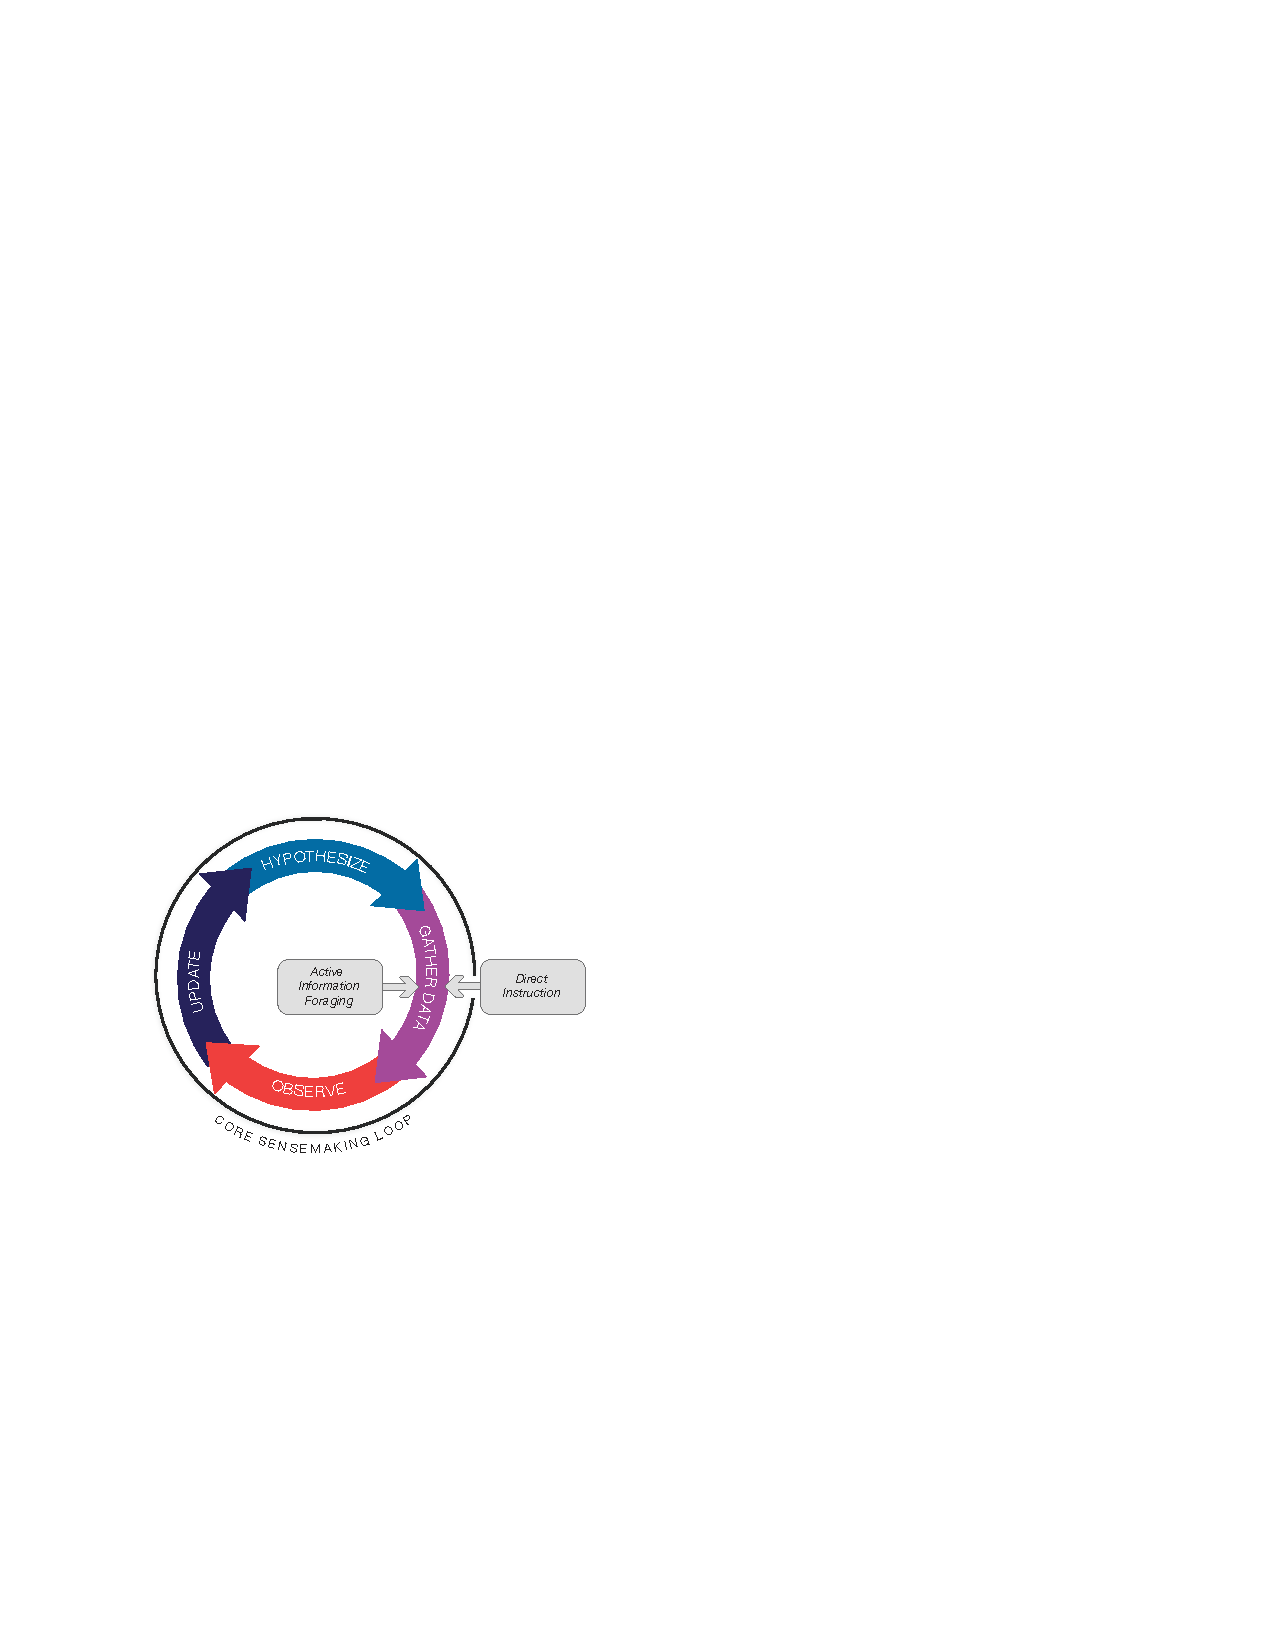
\includegraphics[width=0.45\textwidth]{figures/sensemaking_loop}
  \caption{The sensemaking loop depicts the successive cognitive process that are 
engaged when attempting to derive a meaningful understanding of an initially 
ambiguous situation. The stages of the loop closely mirror the process of scientific 
reasoning engaged by scientists. However, a similar set of inductive processes are 
at play in many real-world situations (e.g., working an unfamiliar ATM machine, 
reading a complex nutrition label).}
  \label{fig:sensemaking_loop}
\end{figure} 

%While the sensemaking loop just described is fairly abstract, the goal of the 
%present study is to test and elaborate this theory with the aim of better 
%understanding how to structure formal and informal learning experiences in 
%developmentally appropriate ways. 
% JOURNAL
This basic sensemaking framework can be instantiated as a computational 
information processing model \cite{Gureckis:2012,Gureckis:2009,Markant:2012}. 
The advantage of this formal model is that it allows detailed, testable predictions 
about behavior. The model-based theory suggests possible bottlenecks that might 
serve as developmental limitations on learning. For example, young learners may be 
able to correctly update their beliefs about a set of hypotheses given a set of data, 
but have trouble finding the relevant features in the remaining hypothesis space to guide future information 
search, while older learners may be more proficient at all stages of the process. 
The present study explores the development of the data-gathering and updating 
stages in children, with the aim of developing a more complete understanding of how 
learning abilities change across childhood.

Many of the cognitive skills required for active scientific inquiry follow protracted 
developmental trajectories. For example, in tasks designed to assess scientific 
reasoning abilities, children in the older elementary school years (ages 8-10) often 
have difficulty adopting systematic strategies, such as testing the effects of one 
variable at a time or selecting interventions that will lead to determinate evidence 
\cite{Chen:1999}. Although children in the older elementary school years can be 
taught to engage in these strategies via direct instruction \cite{Klahr:2004,Kuhn:2005}, 
it is notable how difficult it is for them to discover and implement them on their own. 

Despite the lengthy developmental trajectory of children's scientific reasoning 
skills, the roots of these abilities are observable even in the early preschool years. 
For example, in simple causal reasoning tasks, preschool-aged children can 
distinguish confounded from unconfounded evidence to draw causal inferences 
\cite{Gopnik:2001,Kushnir:2005,Kushnir:2007,Schulz:2004}. Preschool-aged 
children also selectively explore confounded evidence in their own exploratory play 
\cite{Cook:2011,Gweon:2008,Schulz:2007}. Thus, preschool-aged children show 
early emerging abilities to explore evidence strategically, distinguish confounded 
from unconfounded evidence, and to engage in causal inference from limited samples.

One reason for the difficulties children show may be that 
active inquiry depends on the coordination of a variety of 
component cognitive processes (belief updating, decision making, hypothesis generation, etc.).  
Inefficiencies in any or all of these interrelated processes may serve as developmental limitations.  
For example, young learners may be able to search efficiently for information given a particular 
set of hypotheses but have trouble updating their beliefs correctly given new evidence.
In this sense active inquiry is like a bicycle: when all the elements are properly functioning
and aligned the bike moves forward.  
However, misalignment of any one component can be catastrophic, and it is reasonable to expect
that knowledge gathering in younger children may suffer greatly even if they are only having trouble
with one stage, such as hypothesis updating.

% this par is repeats earlier sensemaking description:
%For example, according to one popular view, learners must generate 
%possible hypotheses to explain their environment.  They then must engage in 
%decision making to ask questions or more effectively gather additional information.  
%They then must understand the results of these inquiry behaviors and update their 
%beliefs accordingly.  The process then repeats with new hypotheses.  The various 
%stages of this loop closely mirror the process of scientific reasoning engaged by 
%scientists~\cite{Russell:1993,Klein:2006a,Klein:2006b}. However, a similar set of 
%inductive processes are at play in many real-world situations (e.g., working an 
%unfamiliar ATM machine, reading a complex nutrition label).

%update their beliefs about a set of hypotheses given a set of data, but have trouble 
%using the remaining hypothesis space to guide future information search. 

%The present study offers a fine-grained analysis of how question asking develops 
%between the rudimentary abilities of kindergartners and the more sophisticated 
%scientific reasoning skills of older children. 

\nocite{Bonawitz:2010pb}
The present study joins with some recent work which attempts to decompose the 
component processes involved in active inquiry (e.g., Bonawitz \& Griffiths, 2010).  
In particular, we tasked four to ten-year olds to identify a hidden insect in
a simple iPad variant of the classic ``Guess Who?" game. Children asked questions to try 
to identify the hidden insect. Across conditions, we manipulated whether the computer program 
helped children to use the new evidence that resulted from their queries to narrow down the
hypothesis space, or whether children had to use the new evidence to update the hypothesis space
on their own.  Our expectation was that helping children--and in particular younger children--to update their beliefs accurately following the 
receipt of new information would free up cognitive resources and lead to more effective question-asking. 
Interestingly, our results opposed our main hypothesis in that elements which 
ostensibly made our task more difficult actually improved the quality of children's inquiry behavior in both younger and older children.  
This study explores the development of the data-gathering and updating stages in children, with 
the aim of developing a more complete understanding of the learning abilities of young children. First, we review the findings and methods of previous developmental studies of question-asking.
%This work was conducted within the context of an informal science museum
%environment, and we conclude with implications of our findings for the design of
%self-guided educational displays 

\subsection{How the ability to ask revealing questions develops}

Experimental tasks based on the 20-questions or ``Guess Who?" game have often been used to
study question asking and active inquiry with both children and adults.
In the game, the asker (participant) tries to determine a hidden object known
only to the the answerer (experimenter) (e.g., ``What animal am I thinking of?")
by asking a series of yes-or-no questions.
\citeA{Mosher:1966} identified two broad question types commonly used in the game: \emph{hypothesis-
scanning} questions test a single hypothesis (e.g., ``Is it a monkey?''), whereas 
\emph{constraint-seeking} questions attempt to constrain the hypothesis space faster by 
querying features that are present or absent in multiple objects (e.g., ``Is it soft?''), 
but that do not directly identify the answer except by virtue of elimination. 

A classic finding in this literature is that younger children (e.g., aged 6) tend to ask more hypothesis-scanning questions, while older children (e.g., aged 11) use more constraint-seeking  questions, and also 
tend to find the answer after fewer questions \cite{Mosher:1966}. 
One explanation is that only older children have developed the ability to focus on the 
high-level features that group the hypotheses, whereas younger children focus on individual stimuli.
Consistent with this viewpoint, manipulations that help children focus on these higher-level features (such as cuing them with basic level category labels instead of exemplar names 
\cite{Ruggeri:2015front} increase the likelihood that young children will generate constraint-seeking questions (see also Herwig, 1982).
Further, although young children are often relatively less likely than older children to ask constraint-seeking questions, even younger children (ages 7-9) are 
more likely to do so when such questions are particularly informative, such as when the hypothesis space is large and there are several equally probable solutions remaining \cite{Ruggeri:2014,Ruggeri:2015}.
\nocite{Herwig:1982}
% (e.g., Ruggeri \& Lombrozo, 2015; 2015).


 %\citeA{Ruggeri:2015} studied 7-8 year-olds, 9-11 year-olds, and 17-18 year-olds 
%asking questions to identify the cause of an event in real-world scenarios (e.g., Why 
%is a man late to work?). All age groups in that study used more constraint-seeking 
%questions when hypothesis-scanning was unwise: e.g., when the problem had a 
%large hypothesis space or when not all solutions were equiprobable.

The behavioral distinction between constraint-seeking and hypothesis-scanning questions can also be studied from the normative perspective of information gain. In general, the most informative question is one that will eliminate half of the remaining hypotheses. 
 Expected information gain (EIG) has often been proposed as a model of how children might evaluate the quality of possible queries.  For example, \citeA{Nelson:2014} found that 8-10 year-old children can search a familiar structured domain (people with varying gender, hair color, etc.) fairly efficiently, tending to ask about frequent real-world features that roughly bisected the search space. 
 Likewise, \citeA{RuggeriXu:2015} found evidence that children's patterns of search decisions were well-explained in terms of EIG.


%Might children be sensitive to this difficulty, and thus seek to avoid errors by using easily-interpretable hypothesis scanning? Might an intervention that aids with hypothesis updating encourage the use of constraint-seeking questions? 
%In this study, we explore how to alter the relative utilization of constraint-seeking
%or hypothesis-scanning via.... \hl{display element, helping with updating.  Also
%we look at developmental changes.}
Whereas previous work has focused on developmental changes in when children generate informative, 
hypothesis-scanning questions, less prior work has considered possible developmental changes in how 
children make use of the new evidence that their questions reveal. 
In a 20-questions task in which 6-8 and 11-year-olds tried to identify which of 24 common objects the experimenter was thinking of, \citeA{Herwig:1982} presented children with a series of two-alternative forced choice decisions between queries--hypothesis-scanning or constraint-seeking--but did not actually give feedback or update the hypothesis space in response to their choices. Kindergartners and first-graders showed comparable and near chance proportions of hypothesis-scanning versus constraint-seeking questions, while older children (second- and fifth-graders) used more constraint-seeking questions. 
In the 20-questions task in which 8- to 10-year-olds were to identify which of 18 people was the hidden target, and played the game to completion several times for different targets, children were allowed to eliminate hypotheses based on acquired evidence, but were given help by the experimenter if needed, and were thus presumably not allowed to make errors.
\citeA{Ruggeri:2014} did not explicitly represent the hypothesis space in Experiment 1's causal reasoning task (e.g., ``Why was a man late to work yesterday?''), and when ten explicit reasons for being late were given in Experiment 2, they remained in view.  That is to say, the process of hypothesis updating was not scrutinized in these prior studies.
Nonetheless, as described in the discussion of sensemaking, effective active inquiry involves the coordination of multiple cognitive processes--representing the hypothesis space, 
generating an informative query, updating one's representation of the hypothesis space in light of the 
data produced by the query, and so on. As suggested by prior work, hypothesis-scanning questions might 
be easier for young children to generate because they do not require abstracting informative higher level 
features (features to query that group classes of hypotheses together and might allow them to be eliminated 
at once). Yet, another reason why hypothesis scanning questions might be easier for young children is that they produce evidence that is easier for them to process. As a hypothesis-scanning question is answered, children are told directly whether the item they queried is correct or not. If instead children ask about a feature (as in a constraint-seeking question), additional cognitive processing is required--children have to take that new information (e.g., that a hidden animal has antennae) and consider each remaining possible 
exemplar in light of this information (e.g., check if each one has the antennae) and eliminate from the 
hypothesis space any that are ruled out by the new information. This process could be cognitively taxing, 
and also prone to errors. Thus, although constraint-seeking questions are often more informative in 
theory, they might not always be so to young children, particularly if children have difficulty using the 
obtained information to update their representation of the hypothesis space accurately. To address 
these issues, in the present study we manipulated whether children received assistance in updating 
their hypothesis space or had to undertake this process on their own, following the receipt of new 
evidence obtained by their queries. 

%Together this work is consistent with the view that active inquiry behaviors are deeply linked
%to component cognitive processes such the representation of the task or
%the structure of the hypothesis space. 

%The experimental framework used here is a variant of the ``20 questions'' game, in 
%which the asker (participant) tries to ascertain what object the answerer 
%(experimenter) is thinking of (e.g., ``What have I got in my pocket?'') by choosing 
%and asking a minimal series of yes-or-no questions. Variants used in experiments 
%often present a finite set of familiar kinds of objects, such as animals \cite{Ruggeri:2015front} 
%or people \cite{Nelson:2014}, from which the to-be-discovered answer is 
%randomly selected, and some even provide lists of acceptable questions for askers 
%to choose from. Investigating children aged 6-11 years, 

%However, these studies all used hypothesis spaces that were likely familiar to 
%participants to some extent---and likely to a larger extent for older participants. 
%In contrast, the present study introduces a novel, hierarchically-structured 
%hypothesis space in which the concrete features are randomly assigned. 

% The present study differs from that of \citeA{Ruggeri:2015} in several ways, among them being 
%that the present task: 1) is not a causal inference task, 2) introduces a novel 
%hypothesis space with features' informativeness being randomly assigned, and 3) 
%presents the available strategies (i.e., hypothesis-scanning and constraint-seeking 
%queries) explicitly as side-by-side buttons.
%
%In this study, children (ages 5-10) play multiple rounds of a self-guided 20-questions 
%style iPad game with a structured but novel hypothesis space. 

%\hl{todd says: We focus here on belief updating.  That this
%can be a challenge for children to coordinate along with other processes in
%the task (i.e., asking questions).  In addition many theories of active
%information seeking (e.g., information gain) include within the valuation of a
%possible query a belief update step (Coenen \& Gureckis, 2015).  As a result
%one might expect tasks which aid people in performing belief updating might
%also improve their active information seeking.}
%
%\hl{Todd: In our experiment children attempted to play a version of the Guess
%Who? game.  On each trial children could choose to click a button to obtain
%information about a hidden insect.  There were different types of buttons
%available (exemplars which just allowed children to ask if one specific insect
%was the hidden one) or features (which allowed children to ask if a specific
%property applied to the hidden insect).  These two query button types roughly match
%the distinction in Mosher and Hornsby (1966) concerning hypothesis-scanning
%and constraint-seeking questions.  Our primary manipulation was
%to either help children with the updating step by automatically removing
%from the set any insect which is inconsistent with evidence encountered so far.
%Our primary dependent measure what the sequence and type of button
%presses the children made as they learned to identify the insect.}
%\vspace{-.1cm}
\section{Experiment}
%\vspace{-.2cm}
The purpose of the experiment is to investigate how children utilize hypothesis-
scanning and constraint-seeking questions when trying to discover a hidden feature 
in a novel environment, and to ask whether evidence-based belief-updating is a 
bottleneck in the knowledge discovery process. To address these issues, we created 
a tablet-based game in the ``20-questions'' style (or more specifically, ``Guess 
Who?''). Formally, this task involves search of a binary decision tree. To accomplish 
this search optimally, one should search for and query the feature at each step that 
most nearly bisects the hypothesis space. 
We will assess how well  participants monitor their own understanding and how they choose to seek additional 
information until their understanding is complete. Specifically, we ask how children 
test hypotheses when they can use a mixture of hypothesis-scanning and constraint-seeking 
questions in a novel feature space: Do they use feature queries and then scan hypotheses? 
%Do they gradually learn to test more discriminative features? 
Do they make queries that are context-sensitive (i.e., relevant to the information state 
they are currently in)? Does manually updating the hypothesis space reveal 
bottlenecks, or perhaps push learners to find more informative queries?

\subsection{Methods}
%\vspace{-.1cm}
\subsubsection{Participants}

Participants in this experiment were 134 children between the ages of 5 and 10 
years old who were recruited at the American Museum of Natural History's 
Discovery Room. Of the 134 children recruited, we analyze the data from 121 
children (21 5-year-olds, 20 6-year-olds, 22 7-year-olds, 20 8-year-olds, 20 9-year-olds, 
and 18 10-year-olds) who completed 5 or more rounds of the game.

\subsubsection{Stimuli}

On each round, sixteen insects with the same body shape but with varying features were used as stimuli. insects were defined by the presence or absence of 9 features: green body, 
orange eyes, antennae, big spots, tiny spots, legs, leaves, water droplets, and blue 
``fur''. Figure~\ref{fig:example_bugs} shows an example of two of the body shapes used, each with all of the binary features present. One of the sixteen possible insects was chosen as the ``hidden insect" on each trial which 
children attempted to identify by asking questions. The hidden insect was 
randomly selected on each round, and each round had differently-shaped insect 
bodies, selected from a pool of 16 unique body shapes.  The insect task was used to fit thematically with the content of the AMNH Discovery Room activities.


\begin{figure}[h]
  \centering
  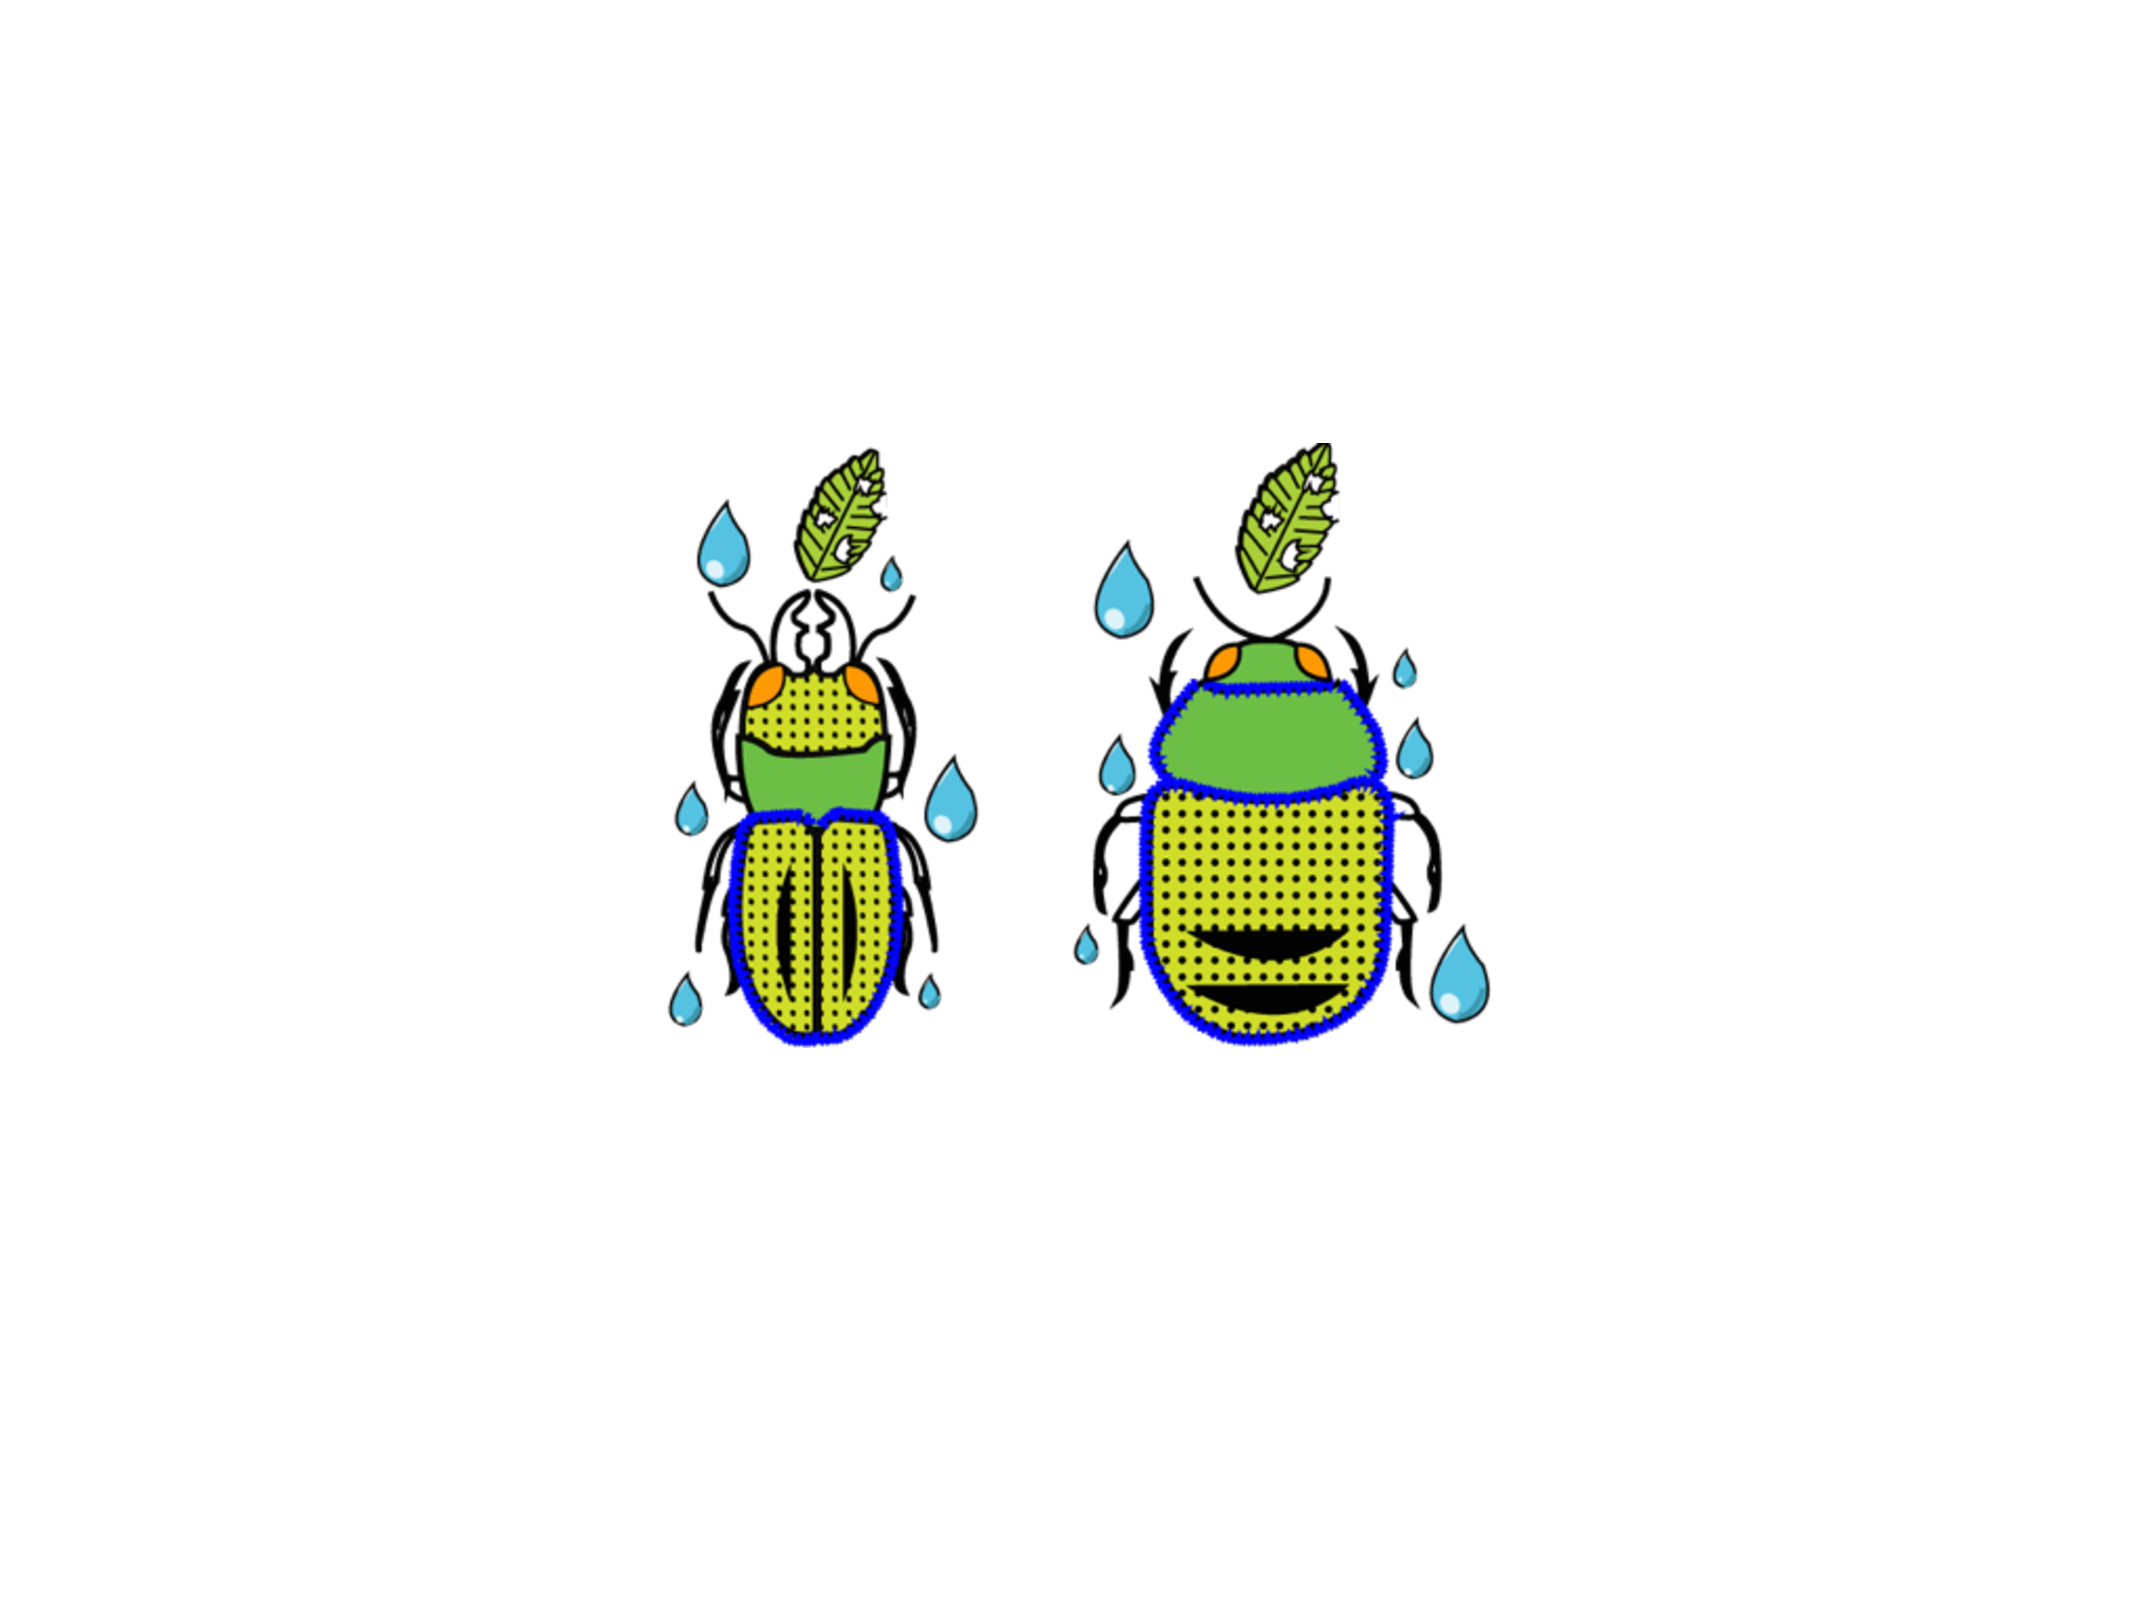
\includegraphics[width=0.4\textwidth]{figures/example_bugs}
  \caption{Examples of two insect types with all 9 of the binary features present. Each round used one of the 16 
body shapes. } % Each insect in a round had a unique combination of features.
  \label{fig:example_bugs}
\end{figure} 

\subsubsection{Design}

Across the sixteen items, some features were more frequent than others (e.g., one was relevant to eight of the  insects), while some were very infrequent (e.g., two were relevant to only two insects), with an
abstract structure shown in Figure~\ref{fig:feature_table}. This introduced
strong differences in the informational utility of each feature.  For example,
given no other information it would be quite informative to ask about feature F1
because it is shared with half of the possible insects.  In contrast, feature
F9 is less informative on the first trial because most of the insects do no have this
feature. The abstract features in Figure~
\ref{fig:feature_table} were randomly assigned to the visual features for each 
participant, and then remained consistent across rounds. This gave participants the 
opportunity to learn the structure across rounds, for example to perhaps figure out 
which visual features are most relevant to ask about first.

\begin{figure}[h]
  \centering
  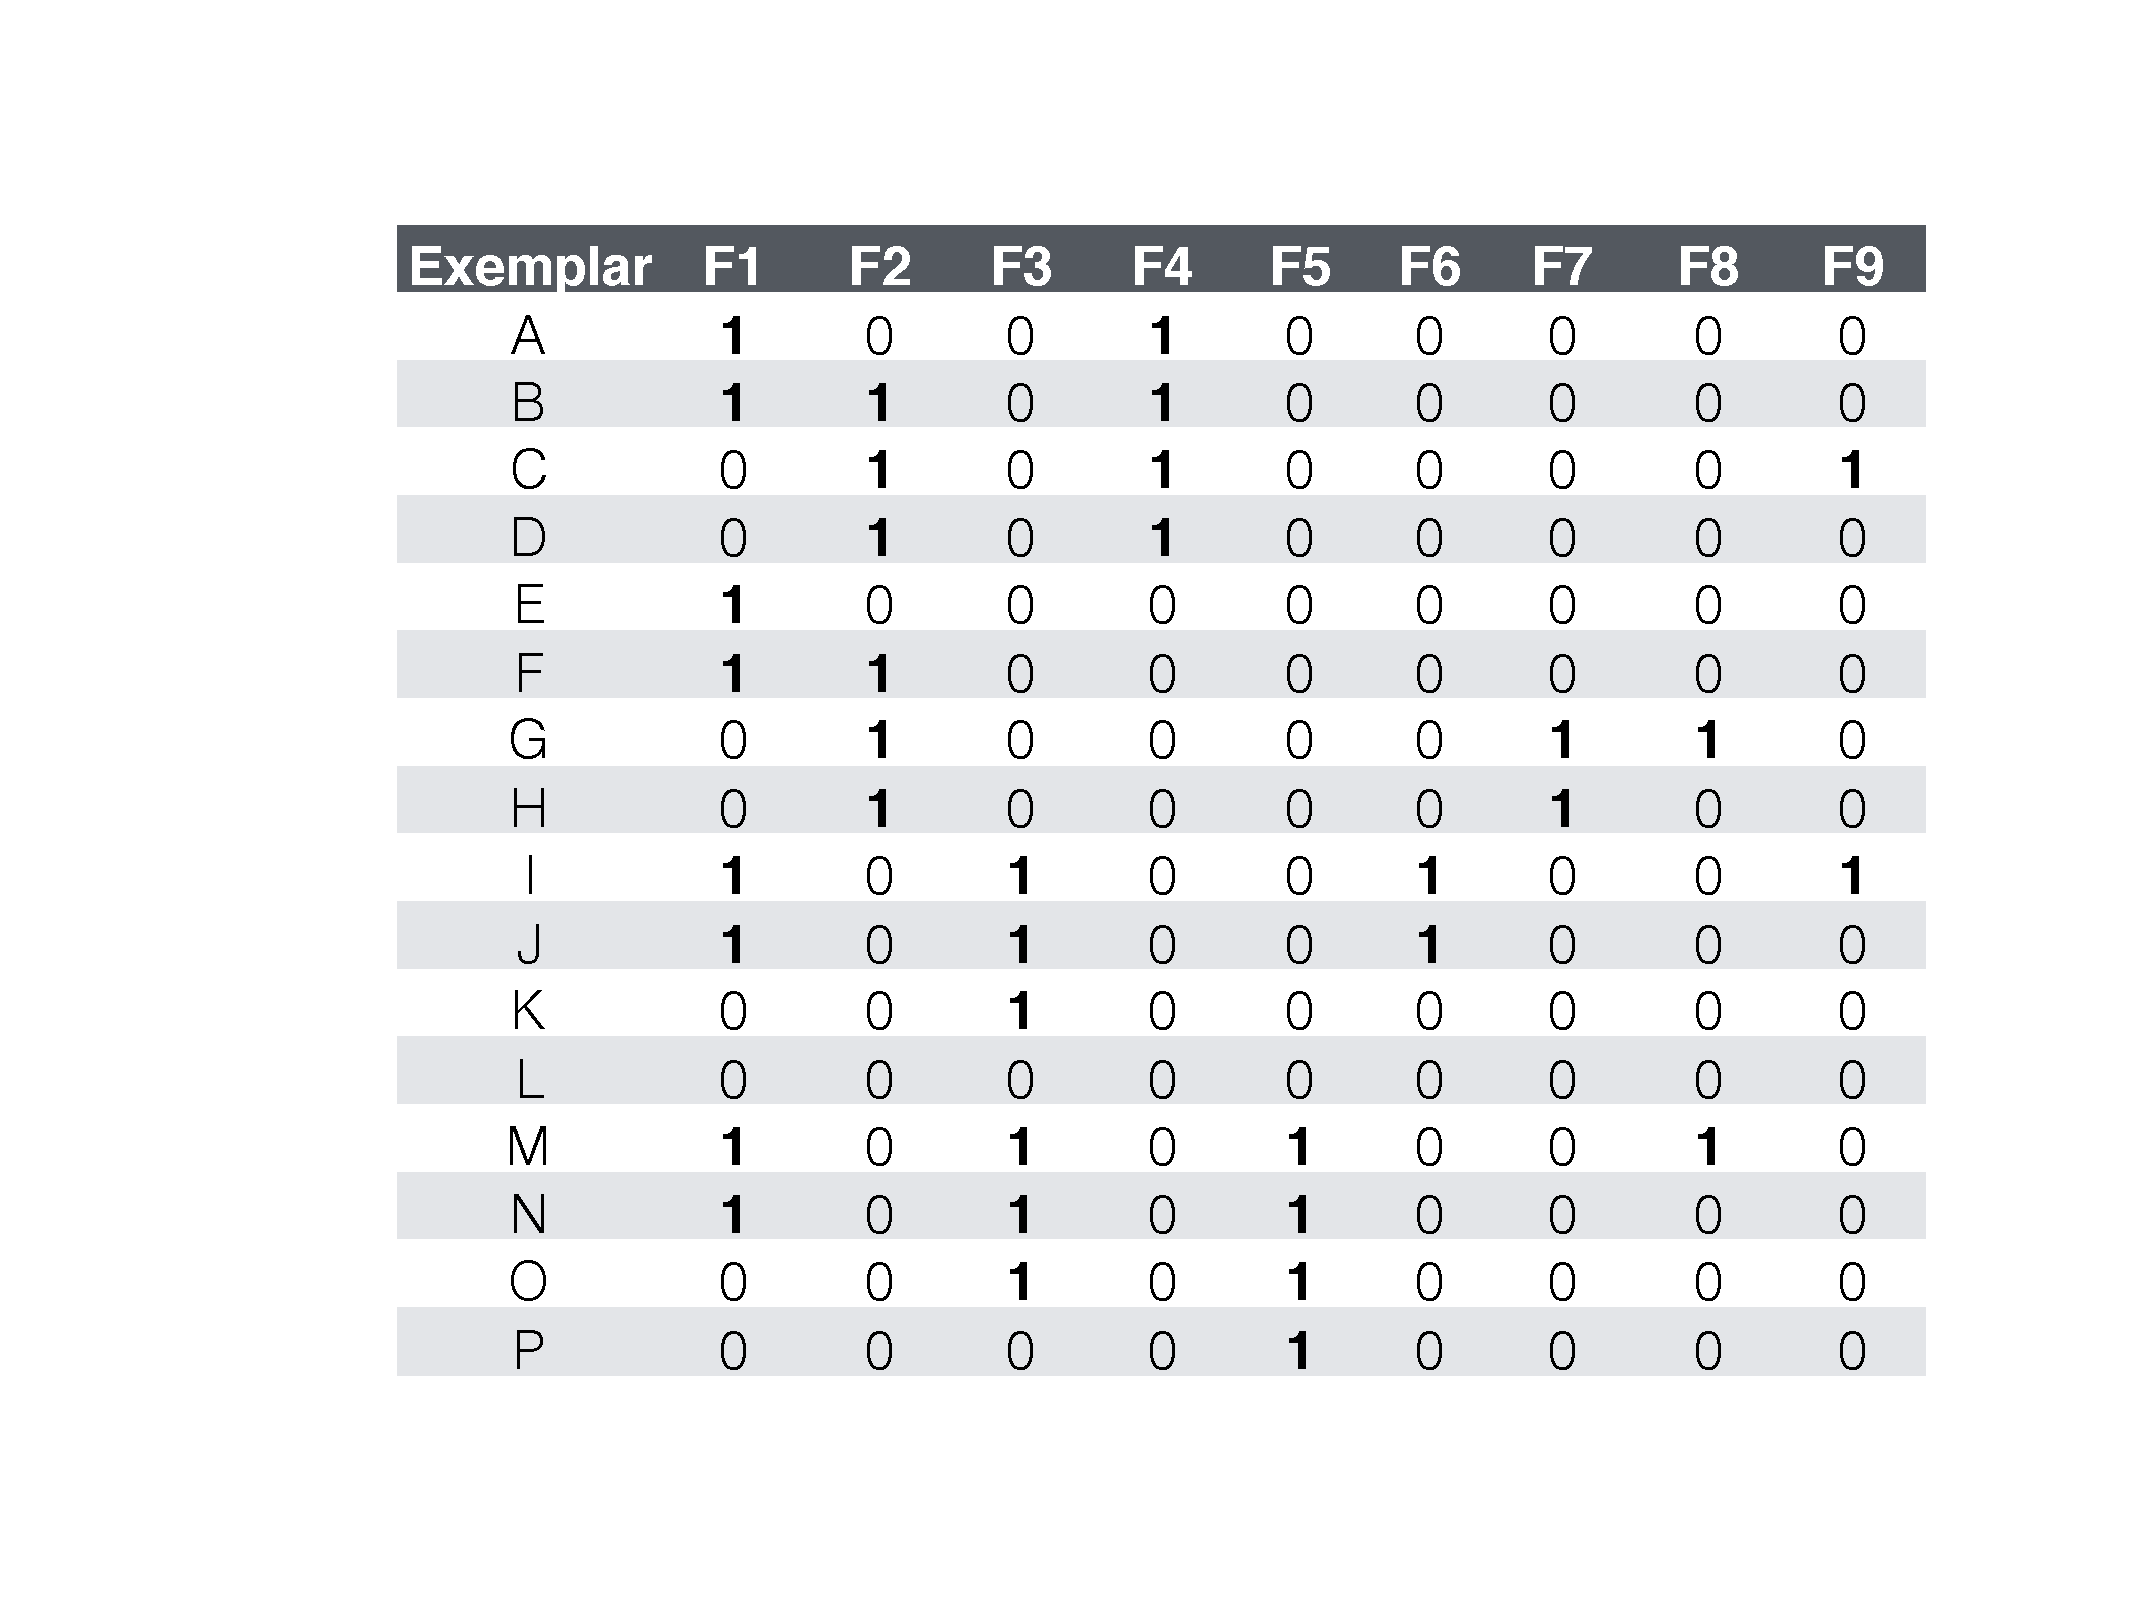
\includegraphics[width=0.55\textwidth]{figures/feature_table}
  \caption{The abstract feature structure of the 16 exemplars used in each round. 
Each participant had these abstract features randomly assigned to the visual 
features, but had a consistent assignment used round-to-round.}
  \label{fig:feature_table}
\end{figure} 

Each of these features was visually represented on a button, available for participants to query. Before 
participants were allowed to begin, the experimenter explained a random selection of at least three of these buttons. 
An additional feature button depicted a particular body shape that was not relevant to the insects on display. 
Instead of choosing a feature button, participants could at any time query an exemplar by tapping it to determine if it was the hidden insect or not. This paradigm thus enables us to investigate both the qualitative strategies used by participants (constraint-seeking feature queries or hypothesis-scanning exemplar queries) and to quantify how efficiently participants search the hypothesis space, within and across rounds as they learn a novel structured stimulus space. Moreover, we introduce a novel manipulation: after making a feature query, participants in the manual-update condition must select the hypotheses that are consistent with the feedback, whereas participants in the automatic-update condition have the hypothesis space automatically updated. This manipulates the ease of updating the hypothesis space: a difficult step in the cycle of active inquiry that has not been well-studied. 

\subsubsection{Procedure}

After being trained by an experimenter on a simpler version of the task with unrelated stimuli\footnote{Download 
full task code and instruction scripts: \texttt{https://github.com/kachergis/bugguess}} (a dog searching dog houses) so that they understood how to query exemplars and features, and how 
to eliminate hypotheses, participants played 5 or more rounds of an iPad game asking them 
to identify which one of 16 insects is hidden under a rug (see Figure~\ref{fig:task-overview}). 
The task alternated between the query phase and the elimination phase, beginning with the 
former. In the query phase, players could either query an individual insect by tapping one (equivalent 
to asking, ``Is this the hidden insect?''), or choose use a feature query button (e.g., the green button asks 
``Is the hidden insect green?'') to find out whether the hidden insect had a particular feature. If a 
single exemplar was queried by tapping on it, feedback was immediate: if it happened to be the 
hidden insect, a smiley face appeared and the round is done, whereas if the tapped exemplar 
was not the hidden insect, a red ``X'' was shown on top of the tapped insect and the insect becomes 
grayed out (i.e., eliminated). After a feature query, the insect gives feedback, saying 
``Yes!'' (it has the feature; narrated by the experimenter), or ``No!'' (it does not have 
the feature). This is followed by the elimination phase, during which insects that are 
inconsistent with the feedback are eliminated, and the hypothesis space is thus narrowed. 

Participants were assigned in counterbalanced order to one of two hypothesis-updating conditions. In the automatic-update condition, after the feedback from a 
feature query, subjects merely pressed the ``Eliminate'' button and all the irrelevant insects 
are eliminated (grayed out), and the game returned to the guessing phase. In the 
manual-update condition, after a subject made a feature query and saw feedback, 
they had to select each insect that was consistent with the feedback for that feature, as 
shown in the top right of Figure~\ref{fig:task-overview}. insects were selected (denoted by a green box) by 
tapping, and could be deselected by tapping again. Only when participants were done 
selecting insects did the experimenter press the ``Eliminate'' button, which eliminated 
any insects that were not selected. 

Although manual-update participants were trained on the process of manual elimination in the 
training task, as well as given gentle reminders in the first round of the insect game, it should be 
noted that it was possible for mistakes to be made during manual updating--unlike in the automatic 
condition. Errors in manual-updating were allowed, and went uncorrected: insects that should have been eliminated but were kept (a `miss') continued to be options, and insects that were consistent with the query but wrongly eliminated (a `false alarm') were grayed out. In the event that the hidden insect was wrongly eliminated during a manual-update error, the round was played out until all of the hypotheses were grayed out. The experimenter would then indicate that the insect must have been mistakenly eliminated (but not at what point), and would end the round by clicking the grayed-out exemplars until the hidden one was found. These final clicks (beyond when all hypotheses were eliminated) were not included in the analysis.

At the beginning of each round, the experimenter would say, ``Let's try to find which insect is hiding pretty quickly, so we can do more!'' Thus, the task mostly relied on intrinsic motivation to solve the puzzle quickly, providing no direct incentive to be efficient. Participants were welcome to complete more than five rounds, if they desired to: after the fifth and each successive round, they were asked, ``Do you want to play again?''

\begin{figure}[!h]
  \centering
  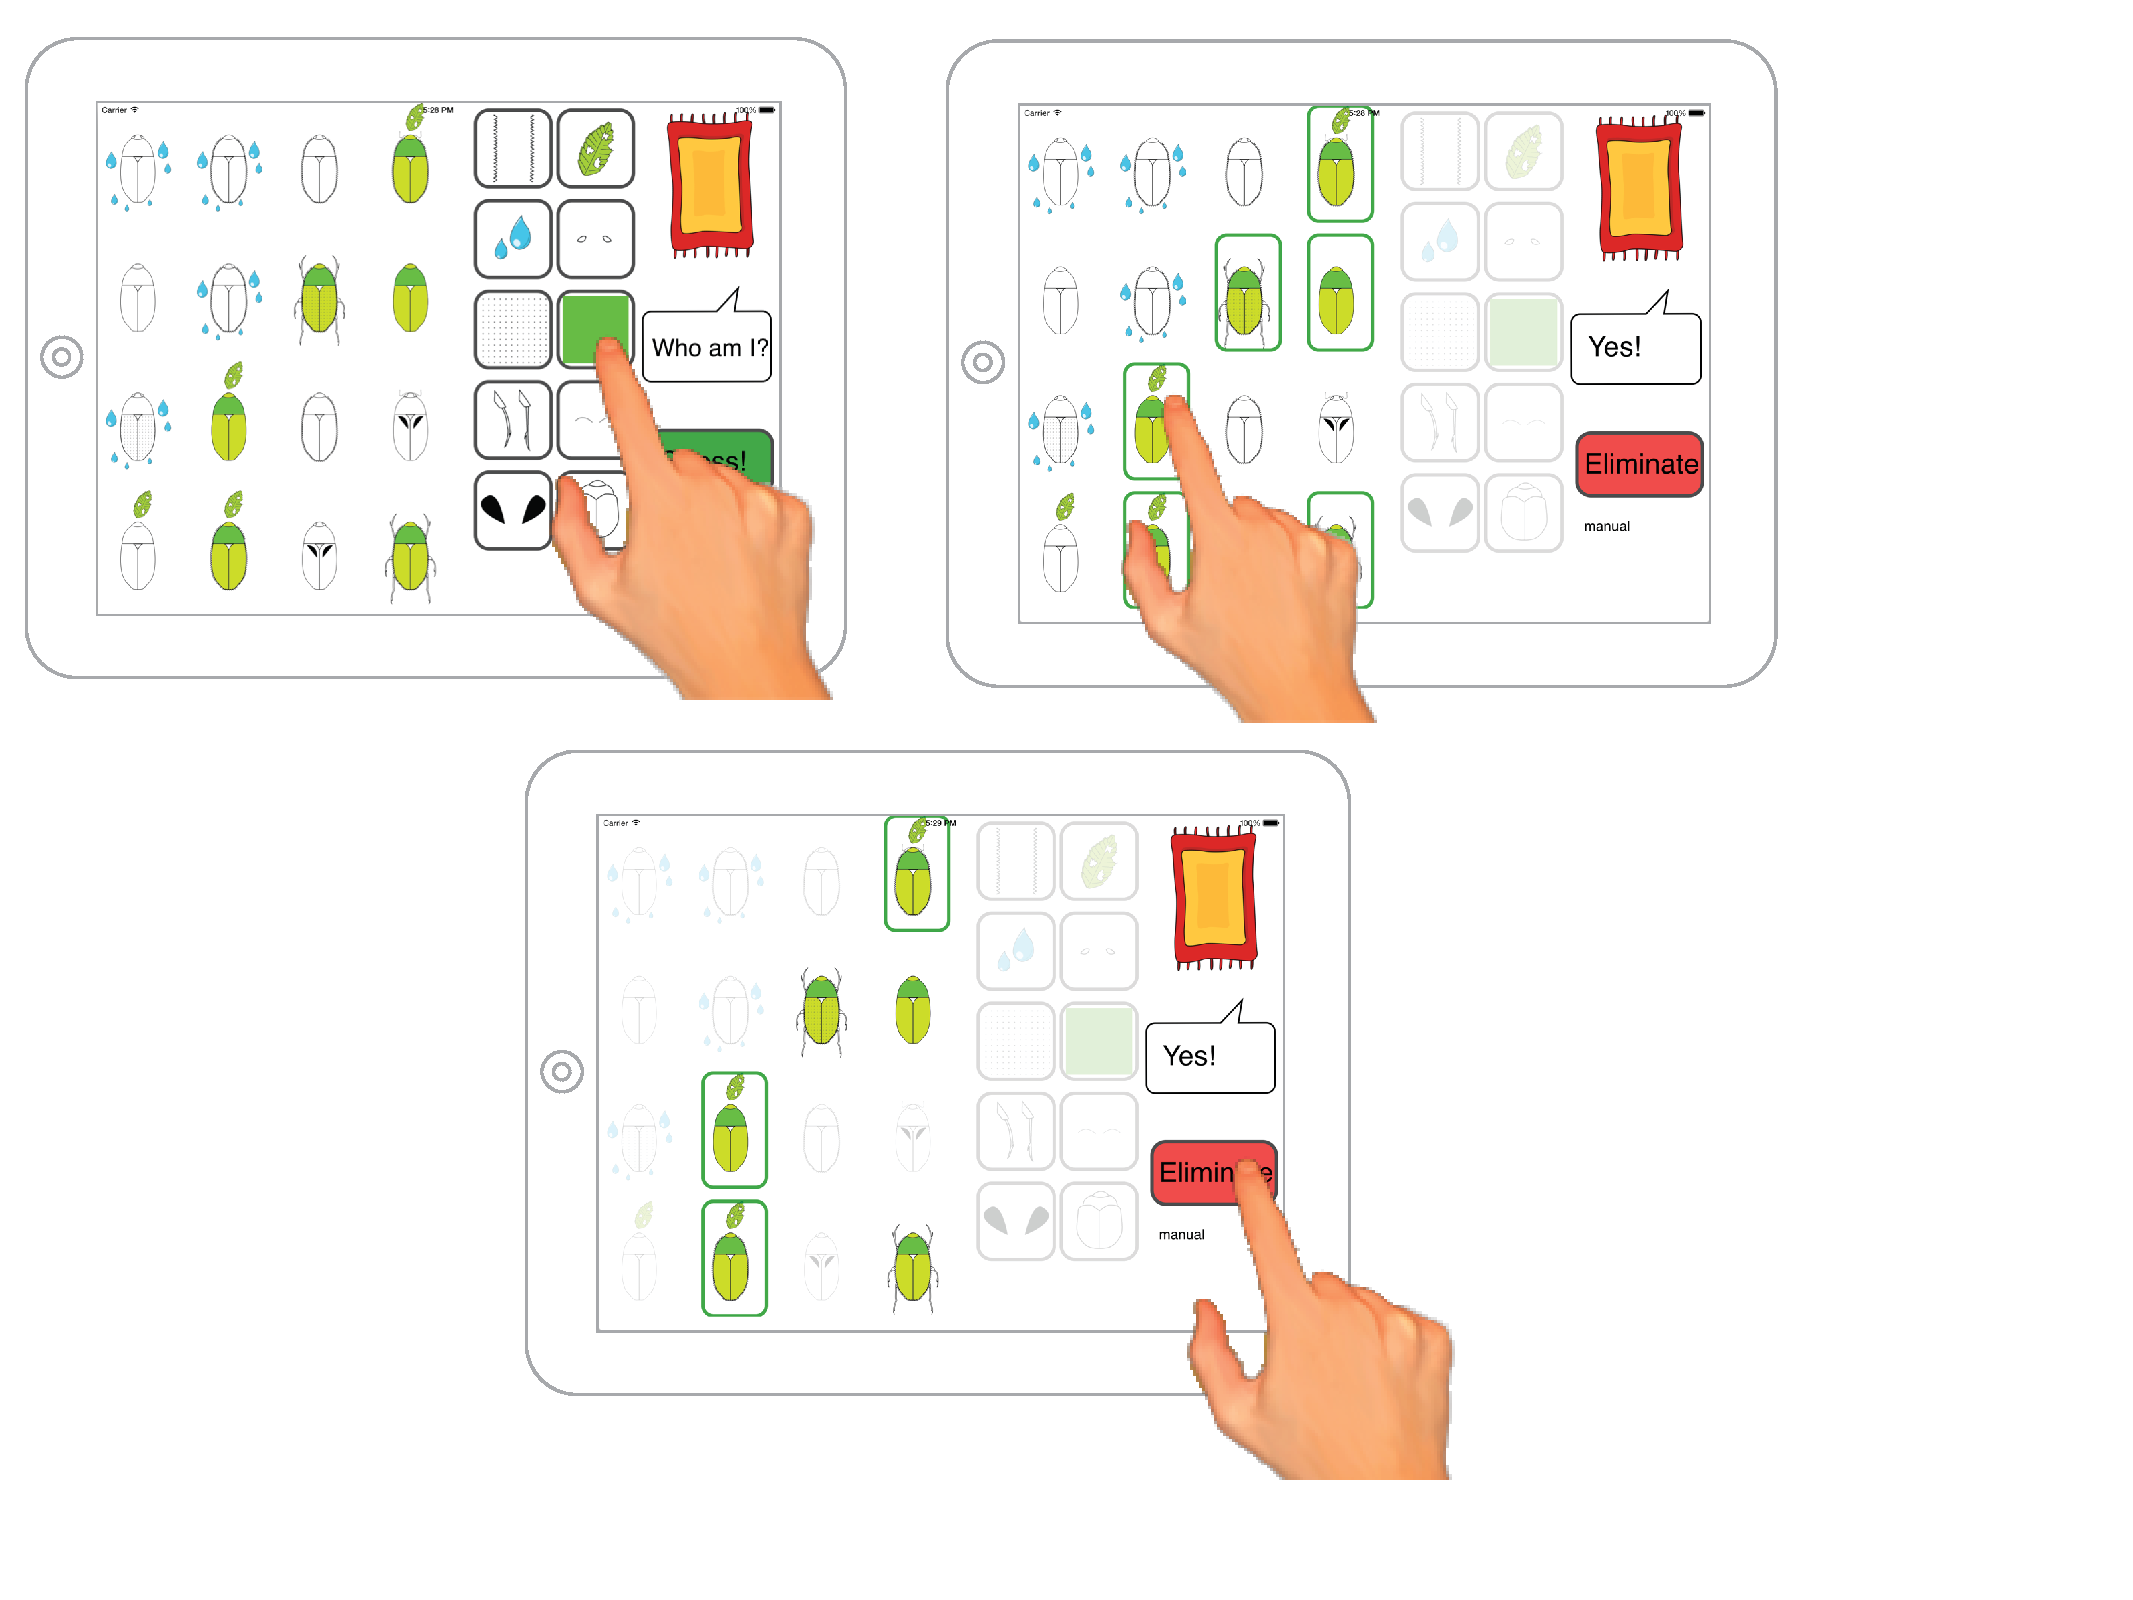
\includegraphics[width=0.7\textwidth]{figures/task_overview}
  \caption{Task overview: in the upper left, a feature button is used, asking if the insect 
hidden under the rug is green. Given feedback (``Yes!''), participants in the manual 
update condition select the insects that are consistent with this new information (upper 
right), whereas in the automatic condition the consistent insects are selected by the 
game. Players in both conditions press the red button to return to the button phase, 
and again either choose a feature button or query a single insect.}
  \label{fig:task-overview}
\end{figure} 


\subsection{Results}

\subsubsection{Overall}
% JEP: General / Cognition 

% - mention that there was no effect of round!
We analyzed only the first 10 rounds of each game (only 8 children played more than 
10 rounds, including one who played 51 rounds). This covers 722 rounds from 121 
children. The mean number of total queries (feature and exemplar) taken to complete a round was 6.5 in the automatic-update condition, and 7.6 in the manual-update condition. Although the median queries to complete a round in each condition was 6, the distributions were significantly different (Kolmogorov-Smirnov test, $D = 
0.13$, $p<.01$). As an appropriate baseline for comparison, we simulated 700 rounds of the game with an agent that clicked
randomly in the task, choosing uniformly at random on the first click from 16 exemplars and 10 feature buttons, and continuing with whatever stimuli (and feature queries) remain after each click, while making no update errors. This random agent took on average 8.9 queries (median: 9) to complete a round---more queries than participants in either condition.

\subsubsection{Qualitative Querying Behavior}

Participants' mean number of queries per round were subjected to an ANOVA with update condition 
(automatic vs. manual) and age group (5-7 vs. 8-10) as between-subjects factors and query type as 
a within-subject factor. This analysis indicated significant main effects of condition (F(1,229) = 4.60, $p<.05$) 
and age group (F(1,229) = 12.20, $p<.001$), and no significant main effect of query type 
(F(1,229) = 0.10, $p=.75$). Overall, older children required fewer queries of either type to complete a 
round ($M_{5-7} = 4.2$, $M_{8-10} = 3.3$), also evidenced by a significant negative correlation 
with age ($t(119) = 3.24$, $p=.001$, $r=-.28$). There were significant interactions of condition 
and query type (F(1,229) = 22.18, $p<.001$), and age group and query type (F(1,229) = 12.25, 
$p<.001$), detailed below. No other interactions were significant (all F-values $<1$).  
In comparison to the manual condition, 
there were fewer exemplar queries in the automatic condition ($M_{man} = 5.0$, 
$M_{auto} = 3.2$, $t(103.5)=4.1$, $p<.001$), while there were more feature queries 
in the automatic condition ($M_{auto} = 3.8$) ($M_{man} = 3.3$, $t(102.9)=2.1$, 
$p<.05$).
These query rates are all lower than the simulated random rounds' mean number of feature queries (6.5) and exemplar queries (5.3), but above the optimal.\footnote{Note that although there are at first more exemplars (16) than feature buttons (10), after the first click or two there will likely be few 
exemplars remaining to click, which is why the expected number of exemplar 
queries is lower than the expected number of feature queries in the simulation.} 

Figure~\ref{fig:clicks-per-agecond} shows the average number of query types used per 
round for participants by age group. Both age groups in the manual-update condition used 
more exemplar queries than feature queries, and older participants in both conditions use fewer exemplar queries than younger participants ($M_{5-7}=4.8$, $M_{8-10}=3.0$, $t(119.0)=4.00$, $p<.001$). Older participants used a greater proportion of feature queries than younger participants in both the automatic ($M_{5-7}=.50$ vs. $M_{8-10}=.66$, $t(57.2)=3.12$, $p<.01$) 
and manual conditions ($M_{5-7}=.39$ vs. $M_{8-10}=.50$, $t(50.3)=2.30$, $p<.05$). Thus, both 
conditions replicate the \citeA{Mosher:1966} finding that older children use a greater proportion of 
constraint-seeking questions. 

\begin{figure}[h]
  \centering
  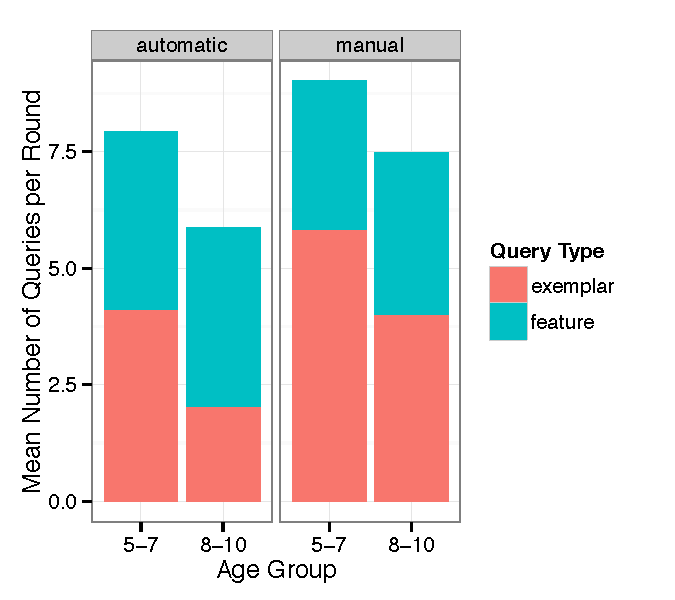
\includegraphics[width=0.55\textwidth]{figures/clicks_by_ageGroup_condition_query_type}
  \caption{Mean number of queries of each type per round by age and condition. Older children use fewer exemplar queries than younger children. Manual-update participants used more exemplar queries and fewer feature queries than automatic-update participants.}
  \label{fig:clicks-per-agecond}
\end{figure} 

The influence of hypothesis-update condition on the number queries used---more feature queries in the automatic condition and more exemplar queries in the manual condition---begs further investigation: are participants reluctant to use feature queries in the manual condition because of the difficulty of updating the hypothesis space? When manual-update participants do use a feature query, do they think more carefully about which feature they choose? We investigate response times in each condition to reveal how much care and thought participants are putting into making each type of query.

% \begin{figure}[!h]
% \centering
%  \includegraphics[width=0.5\textwidth]{figures/query_type_prop_by_round}
%  \caption{Proportion of feature vs. item queries by round.}
%  \label{fig:query-prop-round}
% \end{figure} 
 % \vspace{.05cm}
  
 
\subsubsection{Response Times}

Participants' median RT for each button type (feature and exemplar) was computed and these data were subjected to an ANOVA with condition (automatic, manual) and age group (5-7, 8-10) as 
between-subjects factors and button type as a within-subject factor. There
were significant main effects of button type (F(1,229) = 42.52, $p<.
001$) and condition (F(1,229) = 4.14, $p<.05$), but not a significant main effect of age group (F(1,229) = 0.73). On average, participants took longer to make queries in the manual 
condition (4800 ms) than in the automatic condition (4000 ms). Overall, participants took much 
longer to make feature queries (7,470 ms) than to press an exemplar button (2,680 ms), 
perhaps indicating more thought before making more complex queries. There was also a significant 
interaction effect of query type and condition (F(1,234) = 11.85, $p<.001$). Figure~\ref{fig:basic-rt} shows 
the mean of subjects' median RTs for each query type, split by condition. Feature queries were 
slower in the manual-update condition (7900 ms vs. 5430 ms in automatic), which could indicate 
1) more careful thought given to features in this condition, and/or 2) general hesitance to use feature 
queries, perhaps because it is time-consuming (even difficult) to manually update hypotheses. 
Exemplar queries were faster in the manual-update condition (1850 ms vs. automatic: 2570),
which could be greater readiness to use the simpler strategy. Other interactions were not significant (all F-values $<1$).

\begin{figure}[h]
  \centering
  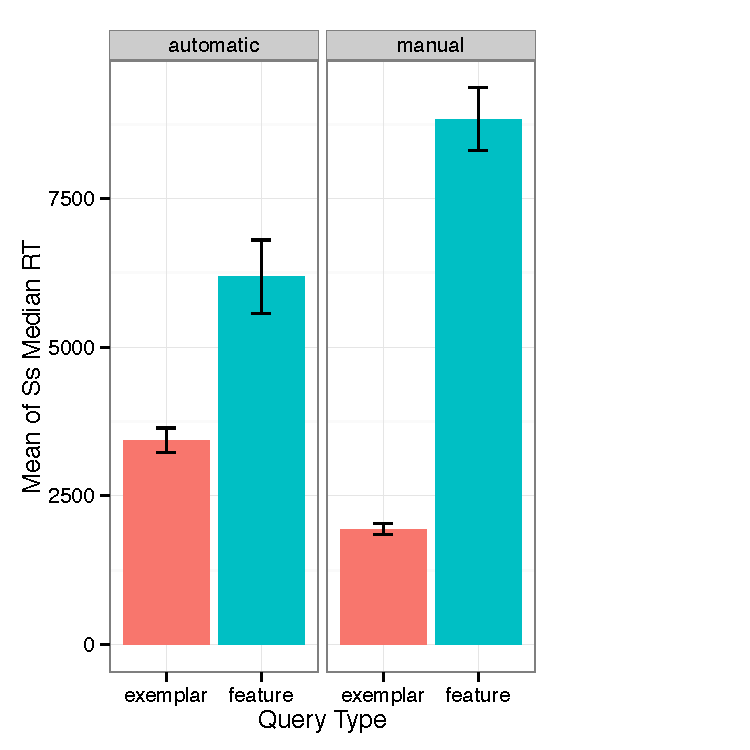
\includegraphics[width=0.55\textwidth]{figures/RT_by_condition_query_type}
  \caption{Mean of participants' median RT for each condition and query type. 
Exemplar queries were faster than feature queries, which represent a more complex 
strategy and thus likely required more thought. Feature queries were slower in the 
manual-update condition: it seems the difficulty of updating in this condition made 
participants think even more carefully about using feature queries. Error bars show 
+/-1SE.}
  \label{fig:basic-rt}
\end{figure} 

 In summary, it is clear that the manual-update condition results in fewer feature 
queries and more reliance on exemplar queries. 
Manual-update participants may be loathe to use feature queries for at least two reasons: 1) it demands more time and cognitive effort to manually update the hypothesis space after a feature query than 
in the automatic-update condition, and 2) the manual update process is error-prone (see below analysis), 
and any mistakes may in turn lead to more exemplar queries in order to recover.\footnote{If the correct answer is mistakenly eliminated, exemplar queries are needed to find it and finish the round. These additional exemplar queries were excluded from analysis.} Therefore we proceed to investigate errors in manual updating, as well as information theoretic analyses that will indicate whether the quality of feature queries varied in the two update conditions. Although the qualitative analyses have thus far revealed interesting effects that build on the previous literature, as the game unfolds the utility of different query types (and specific queries) changes, and can be best quantified using a more sophisticated model-based approach to understanding the quality of children's question asking.

\subsubsection{Manual Update Mistakes}

% make it clear the queries beyond normal round length are removed from analysis
The manual-update condition allows participants to commit two types of error during 
hypothesis updating: a miss is defined as a failure to eliminate a insect, and a false 
alarm is a failure to keep a hypothesis that was consistent with the query. Note that 
a miss is an error of commission--i.e., the insect had to be tapped to be kept--whereas 
a false alarm is an error of omission (i.e., failing to tap a insect), and thus we expect 
more of the latter. Comparing the manual-update subjects' mean number of errors of 
each type per round, indeed there were more false alarms ($M=6.9$, sd = 1.9) than 
misses ($M=1.8$, sd = 1.3; paired $t(58) = 19.8$, $p<.001$). A MANCOVA to 
determine if error rates were related to age did not find a significant effect for either 
misses (F(1,56) = 0.77, $p>.05$) or false alarms (F(1,56) = 0.23, $p>.05$). Given 
the fairly high rate of errors in manual updating, it is perhaps unsurprising that fewer 
feature queries and more exemplar queries were made in this condition than under 
automatic updating of the hypothesis space. However, RT analyses indicated that 
feature queries took longer under manual updating: is this just reluctance, or could it 
be that feature queries were more carefully considered in this condition than under 
the ease of automatic updating? The expected information gain of children's feature queries provides a measure of their sensitivity to the information structure in the stimuli.

\subsubsection{Expected Information Gain}

Each successive query reduces the size of the remaining hypothesis space to some degree: on the first move, querying the appropriate feature (F1) can cut the space in half. When two hypotheses remain, even an exemplar query will cut the space in half. The appropriate way to analyze the contextual sensitivity (i.e., are they 
choosing a feature that is present for half of the remaining exemplars, thus quickly 
reducing the hypothesis space?) of participants' queries is to calculate the Expected 
Information Gain (EIG) of the query they made. We first introduce key terms used to 
define EIG. Entropy measures uncertainty about the outcome of a random variable 
$X$. Entropy is 0 when there is only one possible outcome, and maximal when all 
possible outcomes are equiprobable (i.e., a uniform distribution).

\begin{equation}
  H(X) = -\sum_{x} p(x) \cdot log(p(x))
\end{equation}

Mutual information gain measures the change in entropy as we receive a new piece 
of information $Y$, i.e., how much does our uncertainty about X change given that 
we know Y?

\begin{equation}
  I(X;Y) = H(X) - H(X|Y)
\end{equation}

The Expected Information Gain (EIG) of a query $Q$ is the weighted average of the 
information possible from each possible answer to the query, weighted by the 
current probability of receiving that answer. This will be 0 (or near-0) for queries that 
can be expected to eliminate none or just one or two hypotheses in a large space, 
and more positive for queries that are likely to eliminate a larger number of 
hypotheses. In this task, EIG is maximal (1) for a feature query that will eliminate 
half the remaining hypotheses. Such a query is always available at the beginning of 
any round, and due to the partially-nested feature structure used, maximal EIG 
queries are often available at other stages of the round.

\begin{equation}
  EIG(Q) = -\sum_{Y} p(Y|Q) I(X;Y)
\end{equation}

% moved discussion of EIG use to study children's decisions to intro
In our study, the EIG for each participants' feature queries\footnote{Exemplar query EIGs are 
less interesting, as they are a simple function of how many remaining hypotheses 
there are. Participants' choice of feature query, on the other hand, indicates how 
sensitive they are to the relevance of each feature--and to the context of their 
current situation.} were computed, and their mean EIG was 
subjected to an ANOVA with condition and age group (5-7 vs. 8-10) as between-subjects factors. 
This ANOVA indicated significant main effects of condition (F(1,115) = 55.0, $p<.001$) 
and age group (F(1,115) = 12.42, $p<.001$), with no significant interaction effect (F(1,115) = 0.2, $p>.05$).\footnote{The same significant effects and similar mean EIG values were obtained when analyzing only the first two feature queries per round, when manual- and automatic-update participants were on more equal footing (i.e., before further manual errors--which could raise or lower the EIG of the remaining feature queries).}
Figure~\ref{fig:EIG_by_age} shows mean EIG per feature query by age group and condition, along with the appropriate baseline for comparison: a simulation based on the subjects' data, but showing the mean EIG of all the feature queries (i.e., as if subjects had chosen randomly). Note that randomly-chosen features for the manual-update subjects have a higher EIG than for automatic-update subjects (perhaps driven by update errors quickly reducing the hypothesis space--although the reverse could happen, too), the simulated random EIGs are far below the corresponding human data.
Mean EIG of feature queries for each subject was marginally significantly correlated with 
age ($t(116)=1.77$, $p=.08$, $r=.16$), showing that older children tended to use more relevant feature queries. 
The feature queries made by participants in the 
automatic condition had significantly lower EIG than those made in the manual 
condition ($M_{auto} = .60$, $M_{man} = .74$, $t(116) = 5.49$,  $p<.001$). Thus, 
although manual-update participants used fewer feature queries overall, and tended 
to make mistakes during hypothesis updating, the greater amount of time they spent 
when choosing a feature query tended to pay off: manual-update participants 
queried features with higher expected information gain than automatic-update 
participants. Indeed, there was a weak but significant correlation of participants' mean feature query RT and EIG ($r=.20$, $t(116)=2.17$, $p<.05$), verifying that longer RTs are associated with more informative feature queries.
% information gain conditioned on what they know? (duplicate feature clicks?

\begin{figure}[t]
  \centering
  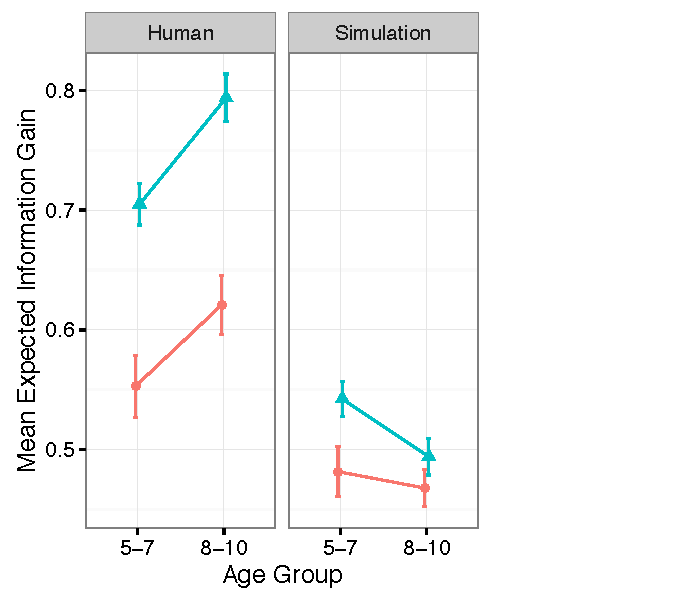
\includegraphics[width=0.55\textwidth]{figures/EIG_by_ageGroup_n_condition_with_random_sims}
  \caption{Mean expected information gain for feature queries by age group and condition, 
with a simulation making random feature queries--in the same situations as subjects (not the earlier random agents)--for comparison. Manual-update subjects had higher EIG than automatic-update subjects, and both were better than random--but suboptimal (1). Older children had higher EIG than younger children. Bars show +/-1SE.}
  \label{fig:EIG_by_age}
\end{figure} 

\subsubsection{Click-by-click behavior}
%Individual strategies: mostly exemplar vs. feature queries? 

Do participants start a round by making a feature query? After how many feature 
queries do they switch to making exemplar queries? Figure~\ref{fig:query-prop-click} shows the mean proportion of feature vs. exemplar queries by click index within a round for each update condition split by age group, contrasted with simulated agents choosing any available buttons uniformly at random throughout the game. Older children show a much higher proportion of feature queries in the first three clicks of the automatic condition, and the first two of the manual condition. In both update conditions, the first three clicks are more likely to be feature than exemplar queries, and automatic-update subjects often make a fourth feature query before likely moving to exemplar queries. 
Both human conditions are quite different than the simulated random agent. 
Rather, the response profile of human participants looks generally like the optimal sequence: 3 feature queries and then one (sometimes two) exemplar queries. However, as was shown earlier, participants rarely chose the most informative feature to query at any given time, and manual participants made a number of updating errors. Where does the higher EIG for manual-update feature queries come from? Are they choosing the best feature query from the start, or are they simply better at testing more contextually-relevant features later in the round?

Figure~\ref{fig:EIG_by_click} shows mean EIG of feature queries by click index (ignoring exemplar clicks), with a simulation based on the participants' data for comparison: although following the same sequence of situations as participants, this simulation shows the EIG if a feature query had been chosen at random in each instance. 
Figure~\ref{fig:EIG_by_click} reveals that people in the two update conditions had similarly informative first queries--especially for the 5-7 year-olds, who were not much better than random, but that manual subjects' subsequent few feature queries were more informative than automatic subjects' or the random choices. That is to say, manual-update participants chose feature queries that were more contextually appropriate for the particular set of remaining hypotheses, in contrast to automatic-update participants who--despite finding an informative feature for the first query--paid less attention to the unfolding situation. In fact, after the initial high-quality query, the younger automatic-update participants chose queries with nearly the same EIG as the random simulation, implying that they more or less ignored the features of the remaining hypotheses. For older automatic-update participants, feature query EIG was better than random after the first query, although it remained below manual-update EIG across feature queries.
%Feature queries are made at a rate that is correlated with the number of exemplars 
%they are relevant to ($r=.79$, $t(8)=3.6$, $p<.01$). 

\begin{figure}[!h]
  \centering
  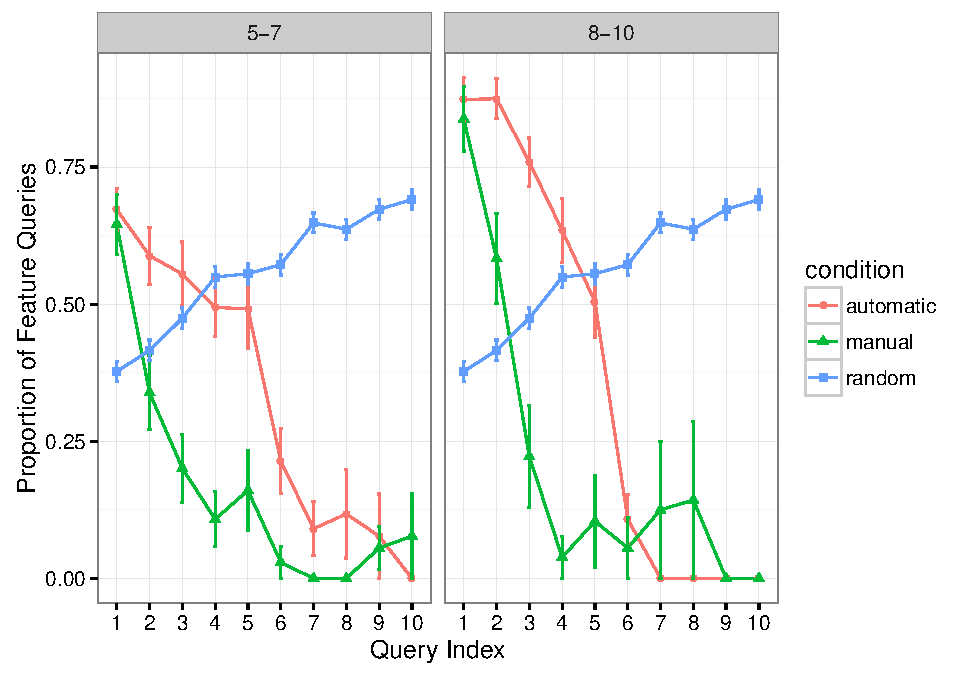
\includegraphics[width=0.75\textwidth]{figures/proportion_feat_queries_by_click} % 
  \vspace{-.1cm}
  \caption{Proportion of feature vs. exemplar queries by click for each update condition, with a randomly-clicking agent for comparison. People in both conditions are more likely to make feature queries rather than 
exemplar queries in the first three clicks of a round, but manual-update participants 
move more quickly to exemplar queries, and are overall more likely to make 
exemplar queries. Older children make a higher proportion of feature queries in the first few clicks of both conditions.}
  \label{fig:query-prop-click}
  \vspace{-.1cm}
\end{figure} 

 \begin{figure}[!h]
 \centering
  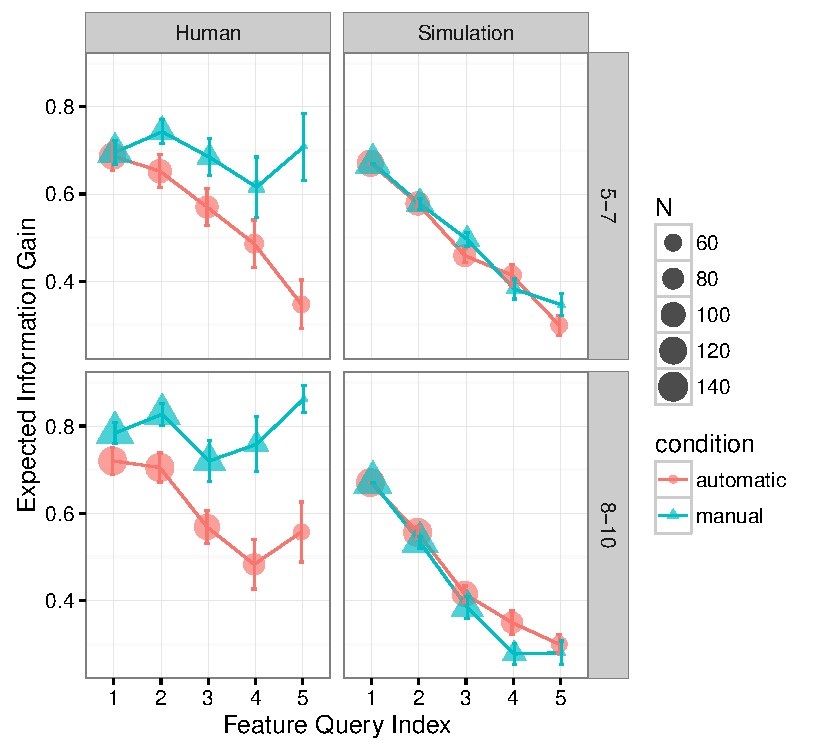
\includegraphics[width=0.55\textwidth]{figures/info_gain_by_click_n_age_w_sims} % info_gain_by_click_w_sim_w_N
  \caption{Subjects' mean expected information gain (EIG) of feature queries by click index (ignoring all exemplar clicks) by condition, with symbol size indicating frequency of occurrence. Although the first feature query--made when the full hypothesis space is possible--had nearly the same mean EIG in both conditions, the next few feature queries in the manual-update condition had higher mean EIG than the automatic condition. This suggests that manual-update subjects paid more attention to the remaining hypotheses after the first query, and made subsequent feature queries that were sensitive to the current context. Making four or more feature queries in a given round was quite rare, as most participants mostly switched to exemplar queries after the second or third feature query. Bars show +/-1SE.}
  \label{fig:EIG_by_click}
 \end{figure} 


\section{General Discussion}

The present study asked children 5-10 years of age to learn feature distributions in an unfamiliar hypothesis space, and examined both their qualitative questioning strategies, and how efficiently they were able to search that space. Previous studies have examined question asking in somewhat familiar hypothesis spaces \cite{Herwig:1982,Mosher:1966,Nelson:2014,Ruggeri:2014,Ruggeri:2015}, but no study we are aware of has considered the step of updating the hypothesis space when new evidence is received--let alone in a novel hypothesis space. In many previous developmental studies, experimenters help children update the remaining hypothesis, quite reasonably: this step is potentially quite challenging, especially for younger children.  Importantly, we manipulated the support children were  given while updating the hypothesis space: after a feature query, participants in the 
automatic update condition were shown which insects were eliminated at the press of 
a button, whereas manual update participants were required to select the insects that 
were consistent with the feedback. 

In line with previous research \cite{Mosher:1966,Ruggeri:2014}, the present study found older children (ages 8-10) asked a higher proportion of constraint-seeking questions than younger children (ages 5-7), who relied more on hypothesis-scanning (i.e., exemplar queries), in both conditions. These qualitative analyses also found that children use more constraint-seeking questions (i.e., feature queries) in the automatic-update condition. On the surface then, these children were using a more efficient strategy than the manual-update children. % suggesting...
From this qualitative analysis alone, then, it is tempting to conclude that automatic updating leads to a better querying strategy than manual updating.

However, in terms of expected information gain, a context-sensitive measure of how well a chosen feature bisects the remaining hypothesis space, it turned out that children in the 
automatic-update condition made less informative feature queries. We 
suggest that the greater mental effort required by manual updating actually lead 
to more careful consideration of which feature query to use, and ultimately a better choice. Indeed, response times for feature queries were slower under manual updating, indicating that greater thought went into making those choices, corroborated by the fact that slower feature query RTs were correlated with more informative queries. Within-round analysis found that automatic-update participants were likely to make feature queries for the first few clicks, while manual-updaters switched often switched to exemplar queries after one (5-7 year-olds) or two feature queries (8-10 year-olds). In terms of quality, feature queries in both update conditions were similar for the first query in a round--and better than the simulation. However, manual-update subjects made more contextually-sensitive feature queries after the first query, whereas automatic-update participants looked much like they were choosing random feature queries, without regard for the current hypothesis space's features. In both conditions, older children made more informative feature queries, but even 5-7 year-olds asked far more informative questions than a random simulation, showing some efficiency in navigating an unfamiliar domain even after only a few minutes of experience. 

In summary, this study provides evidence that hypothesis updating is a difficult, error-prone step in the active inquiry process. Moreover, children are sensitive to the difficulty of this step: if aided in hypothesis updating, they will ask more constraint-seeking questions than if they must manually update the space. However, we also uncovered evidence of a desirable difficulty in this step: manual updating resulted in more informative, contextually-sensitive constraint-seeking questions than the supported update process. Future work will aim to reduce errors in manual hypothesis updating and discover other bottlenecks--or desirable difficulties--in active inquiry. 

Finally, it is worth noting that this partially self-guided iPad study was conducted in the relaxed learning environment of the American Museum of Natural History's Discovery Room. 
Children's developing abilities to engage in the basic steps of scientific 
 thinking are on full display in such informal science learning environments, such as at 
science and children's museums. Indeed, a central goal of these environments is to 
provide children with hands-on opportunities to learn from their own explorations, to 
enable them to gain active experience with the steps of scientific investigation, to 
discover new knowledge, and to develop enthusiasm for and interest in science 
\cite{Bell:2009,Fenichel:2010}. As a result, informal science 
environments may provide an excellent domain in which to investigate the development of understanding. This study demonstrates that such environs can be suitable and fruitful venues for knowledge discovery not only for children, but for scientists, too.

\section{Acknowledgments}

This work was supported by the John Templeton Foundation 
``Varieties of Understanding" grant to TMG and MR. 
We are grateful to Kathryn Yee and Aja Blanco for data collection.

\bibliographystyle{apacite}

%\setlength{\bibleftmargin}{.125in}
%\setlength{\bibindent}{-\bibleftmargin}

\bibliography{sensemaking_refs}

\end{document}
